% 2011 年安徽卷理科第 10 题：函数 f(x)=a x^m (1-x)^n 在 [0,1] 上的图象。
% 来源 PDF：普通高考/2011/2011安徽理.pdf，SHA-256 83dabf28711e3020c00f9fc73f3bf7be70f65fed94ab6ad5b6a39ac840820c0f。
% 原页：第 1 页（A3 三栏）第 2 栏上部，书页码 643。
% 重绘依据：照原页——曲线自原点 O 陡升，在 x=0.5 略偏左处（约为 x=1/3）取最高点，最高点高度标为 0.5，
%   随后下降并在 x=1 处落回 x 轴；x 轴标 0.5 与 1，y 轴在 0.5 处有一短刻度并标 0.5。
%   取 a=27/8、m=1、n=2 作曲线（此时峰值 0.5 在 x=1/3 处取到），与原页示意一致；不按原页绝对比例。
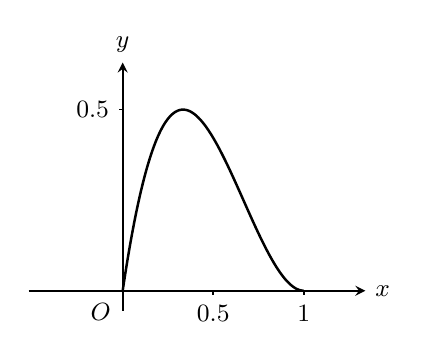
\begin{tikzpicture}[x=2.3cm, y=4.6cm, >=stealth, semithick, font=\small]
  % 坐标轴
  \draw[->] (-0.52,0) -- (1.34,0) node[right] {$x$};
  \draw[->] (0,-0.055) -- (0,0.63) node[above] {$y$};
  % 曲线 y=(27/8)x(1-x)^2
  \draw[line width=0.9pt] plot[domain=0:1, samples=140] (\x, {3.375*\x*(1-\x)*(1-\x)});
  % 刻度与标注
  \draw (-0.018,0.5) -- (0,0.5);
  \node[left] at (-0.02,0.5) {$0.5$};
  \draw (0.5,0) -- (0.5,-0.012);
  \node[below] at (0.5,-0.012) {$0.5$};
  \draw (1,0) -- (1,-0.012);
  \node[below] at (1,-0.012) {$1$};
  \node[below left] at (-0.01,-0.008) {$O$};
\end{tikzpicture}
